\documentclass{article}
\usepackage{amsmath}
\usepackage{amsfonts}
\usepackage{array}
\usepackage{dsfont}
\usepackage{hyperref}
\usepackage{amssymb}
\usepackage{amsthm}
\usepackage{amsfonts}
\usepackage{graphicx}
% \usepackage{geometry}
\usepackage{bbold}
\usepackage{caption}
% \usepackage{pseudocode}
\usepackage{standalone}
% \usepackage[nottoc]{tocbibind}
% \usepackage{apacite}
\usepackage{etoolbox}
% \usepackage{tikz}
% \usepackage{color}
% \usepackage[T1]{fontenc}
% \usepackage{lmodern}
% \usepackage{mathptmx}
% \usepackage{standalone}
\usepackage{accents}
\usepackage{enumitem}

% used for typesetting theorem environments
\usepackage{amsthm}

% used for typesetting tikz graphs
\usepackage{tikz}
% used for typesetting automata using tikz
\usetikzlibrary{automata}


% aaron edit

%wills stuff


\usepackage{tikz}
\usepackage{algorithmic}
\usepackage{algorithm}
\usepackage{verbatim}
\usepackage[super]{nth}

\graphicspath{ {images/} }

\newcommand{\R}{\mathds{R}}
\newcommand{\Zplus}{\mathds{Z}_+}
\newcommand{\N}{\mathds{N}}
\newcommand{\seq}[2][j]{\left\{#2\right\}_{#1=0}^\infty}
\newcommand{\diff}[3][]{\frac{\mathrm{d}^{#1} #2}{\mathrm{d}^{#1} #3}}
\newcommand{\pdiff}[3][]{\frac{\partial^{#1} #2}{\partial^{#1} #3}}
\newcommand{\dd}{\mathrm{d}}
\newcommand{\ip}[2]{\left\langle #1,#2\right\rangle}
\newcommand{\kernl}[1]{\text{ker}(#1)}
\newcommand{\ind}[1]{\mathbb{1}_{#1}~}
\newcommand{\s}{\mathcal{S}}
\newcommand{\Sin}[1]{\sin\left(#1\right)}
\newcommand{\Cos}[1]{\cos\left(#1\right)}
\newcommand{\ubar}[1]{\underaccent{\bar}{#1}}
\newcommand{\argmin}[1]{\underset{#1}{\operatorname{argmin}}\;}

\newtheorem{thm}{Theorem}
\newtheorem{assmp}{Assumption}
\newtheorem{prop}{Proposition}
\newtheorem{lemma}{Lemma}

\newcolumntype{C}[1]{>{\centering\arraybackslash}p{#1}}
\newcolumntype{L}[1]{>{\raggedright\arraybackslash}p{#1}}
\newcolumntype{R}[1]{>{\raggedleft\arraybackslash}p{#1}}

\captionsetup[table]{labelfont=bf}
\captionsetup[figure]{labelfont=bf}

\title{Group 5 Thesis}
\author{Us}

\begin{document}
	\maketitle
	\tableofcontents
	\newpage
	\section{Introduction}
		Imagine an object recorded by a camera and represented in a sequence of 2-dimensional, coloured images. The object may change size due to changes in position (closer to the camera) or even by nature (an inflating balloon). The object may enter a shadow or areas with different lighting causing its brightness and colour to change between images. If the object or the camera moves and rotates, then the location of the object, its shape, and even the background of the object will alter over the sequence of images. Nonetheless, a human could view this sequence of images and associate a region in each image as one object being manipulated. 

		Region tracking in a sequence of images seeks to create a computer program that, given a region in an initial image, can identify the region over subsequent images. The tracking is desired to be achieved even if some characteristics of the region change. This report proposes two distinct applications for such a program: hand-gesture tracking and tracking of anatomical structures of CT/MRI scans. While hand-gesture recognition will process images whose sequence represents change in time, the CT/MRI scan will process images whose sequence represents change along a dimension of the 3-dimensional object that was scanned.

		\subsection{Application: Medical Imaging}
			The main imaging modalities chosen were X-ray Computed Tomography (CT) and Magnetic Resonance Imaging (MRI) scans. These modalities were chosen due to their diagnostic performance and ubiquity of use. For surgeons these scans are an integral portion of planning and preparing for procedures. The ability to automatically segment tissues and render models of them in 3D aids in this process and can also be used to produce implants that fit the patient's anatomy to a greater degree.


		\subsection{Application: Gesture Tracking}
			Following a hand through a video sequence can provide individuals with a touchless interface like the Kinect. Using the cheap an ubiquitous web cam the ability to follow gestures can allow a user to interact more fluidly with technology and prevent interruption of some tasks.

	\section{Prob Def}
		Produce an algorithm that efficiently tracks regions in medical and video sequences with low error.

	\section{Math}
		\subsection{Problem Formulation}
			One of the most important design choices is the initial framing and structureing of the problem. By applying a riggerous mathimatical model to the design problem, a rich body of theory and tools were able to be used and implemented. The framework chosen was that of calculus of variation. This construction ultimatly turns the the problem of region tracking into a funtional minimization problem with convergance garenties. 

			To veiw region tracking under the the light of calculus of variation, some deffintions are needed first. let $\Omega = [0.1] \times [0,1]$ and let every image $I_i$ in the sequence $i\in \{1, 2, ... ,n\}$ be a mapping $\Omega \rightarrow \mathds{R}$. A region $R_i \subset \Omega$ is an element of $2^\Omega$ the power set of $\Omega$. The problem is now structured as finding $R_{l+1}$ given $I_l$, $I_{l+1}$ and $R_l$. To make this problem a functional minimization task, let $E:2^\Omega \rightarrow \mathds{R}$ such that $R_{l+1}$ is the minimizer of $E$.

			\subsection{Mathematical Tools}
				\subsubsection{Euler-Lagrange Necessary Conditions}
					The machinery of calculus of variation bestows the ability to potentially find a minimizer $\gamma^* = \argmin{\gamma \in C}E[\gamma]$. let $C$ be the set of simple closed curves defined as:
					\begin{center}
						$C = \{\gamma: [0,1]\rightarrow\R | \gamma \in \textbf{C}^2, \gamma(0)=\gamma(1),\dot\gamma(0)=\dot\gamma(1)\}$
					\end{center}
					Now define $E$ as a mapping $C\rightarrow\R$ and express it in the form of:
					\begin{equation} \label{eq:einlaform}
						E[\gamma] = \int_0^1{L(s,\gamma(s),\dot\gamma(s))ds}
					\end{equation}
					From optimization it is clear that the first order condition must be satisfied for an $x$ to be the minimizer of some function $f:\R^n\rightarrow\R$. The Euler-Lagrange necessary conditions are the functional analysis equivalent.

					\begin{thm} \label{th:el}
						Let $\gamma \in C$ be a minimizer of $E$ in the form of equation \ref{eq:einlaform} then $\forall s \in [0,1]$:
						\begin{equation} \label{eq:eleq}
							0 = \frac{\partial L}{\partial \gamma}\biggr\rvert_{(s,\gamma(s),\dot\gamma(s))}-\frac{d}{ds}\Bigg(\frac{\partial L}{\partial \dot\gamma}\biggr\rvert_{(s,\gamma(s),\dot\gamma(s))}\Bigg)
						\end{equation}
					\end{thm}
					
					\begin{proof}
						let $\phi$ be an element of $C$ and $\alpha\in\R$. As $\gamma$ is the minimizer of $E$ (implying $E(\gamma)\leq E(\theta)$ $\forall \theta\in C$), clearly $\frac{d}{d\alpha}E[\gamma + \alpha\phi]\rvert_{\alpha=0}=0$.

						\begin{align*}
							0 &= \frac{d}{d\alpha}E[\gamma + \alpha\phi]\rvert_{\alpha=0}\\
							&= \frac{d}{d\alpha}\int_0^1{L(s,\gamma(s) + \alpha\phi(s),\dot\gamma(s)+\alpha\dot\phi(s))ds}\biggr\rvert_{\alpha=0}\\
							&= \int_0^1{\frac{d}{d\alpha}L(s,\gamma(s) + \alpha\phi(s),\dot\gamma(s)+\alpha\dot\phi(s))\biggr\rvert_{\alpha=0}ds}\\
							&= \int_0^1{\frac{\partial L}{\partial \gamma}\biggr\rvert_{(s,\gamma(s),\dot\gamma(s))}\phi(s) + \frac{\partial L}{\partial \dot\gamma}\biggr\rvert_{(s,\gamma(s),\dot\gamma(s))}\dot\phi(s)ds}\\
							&= \int_0^1{\frac{\partial L}{\partial \gamma}\biggr\rvert_{(s,\gamma(s),\dot\gamma(s))}\phi(s)ds}+\int_0^1{\frac{\partial L}{\partial \dot\gamma}\biggr\rvert_{(s,\gamma(s),\dot\gamma(s))}\dot\phi(s)ds}\\
							&= \int_0^1{\frac{\partial L}{\partial \gamma}\biggr\rvert_{(s,\gamma(s),\dot\gamma(s))}\phi(s)ds} + \bigg[\frac{\partial L}{\partial \dot\gamma}\biggr\rvert_{(s,\gamma(s),\dot\gamma(s))}\phi(s)\bigg]_0^1 - \int_0^1{\frac{d}{ds}\bigg(\frac{\partial L}{\partial \dot\gamma}\biggr\rvert_{(s,\gamma(s),\dot\gamma(s))}\bigg)\phi(s)ds}\\
							&= \int_0^1{\frac{\partial L}{\partial \gamma}\biggr\rvert_{(s,\gamma(s),\dot\gamma(s))}\phi(s)ds} - \int_0^1{\frac{d}{ds}\bigg(\frac{\partial L}{\partial \dot\gamma}\biggr\rvert_{(s,\gamma(s),\dot\gamma(s))}\bigg)\phi(s)ds}\\
							&= \int_0^1{\bigg(\frac{\partial L}{\partial \gamma}\biggr\rvert_{(s,\gamma(s),\dot\gamma(s))} - \frac{d}{ds}\bigg(\frac{\partial L}{\partial \dot\gamma}\biggr\rvert_{(s,\gamma(s),\dot\gamma(s))}\bigg)\bigg)\phi(s)ds}\\
							&\Rightarrow 0 = \frac{\partial L}{\partial \gamma}\biggr\rvert_{(s,\gamma(s),\dot\gamma(s))} - \frac{d}{ds}\bigg(\frac{\partial L}{\partial \dot\gamma}\biggr\rvert_{(s,\gamma(s),\dot\gamma(s))}\bigg)
						\end{align*}
						The right hand side of equation \ref{eq:eleq} is continuous and the theorem thus holds for any choice of $\phi$.

					\end{proof}

					The techniques and tools employed in the Euler-Lagrange necessary condition proof provide a viable analogue to the the classic $\R^n$ gradient. Though theorem \ref{th:el} is a powerful result, it is only a necessary condition on the minimum and does not provide a method to find $\gamma^*$.

				\subsubsection{Gradient Decent}	
					Gradient Decent is one tool that has the ability to find critical points of the functional. To begin the $\R^n$ gradient decent schema will be illustrated then extended to the $C$-functional gradient decent system. 

					\begin{thm}\label{th:graddissimp}
						Let $f: \R^n\rightarrow\R$ such that $f$ is differentiable. Let $\nu$ be a mapping $\R^+ \rightarrow \R^n$ defined by:
						\begin{equation}\label{eq:decentsimp}
							\frac{d\nu(x)}{dt}(t) = -\vec\nabla f(\nu(t))
						\end{equation} 
						Then $f(\nu(t))$ is a monotonically decreasing function $\forall t\in\R^+$.
					\end{thm}
					\begin{proof}
						\begin{align*}
							\frac{d}{dt}f(\nu(t)) &= \langle \vec\nabla f(\nu(t)) , \frac{d}{dt}\nu(t)\rangle\\
							&= \langle \vec\nabla f(\nu(t)) , -\vec\nabla f(\nu(t))\rangle\\
							&= -\langle \vec\nabla f(\nu(t)) , \vec\nabla f(\nu(t))\rangle\\
							&= - \|\vec\nabla f(\nu(t))\|^2\\
							&\leq 0\\
						\end{align*}
						thus $f(\nu(t))$ is monotonically decreasing $\forall t\in\R^+$; with equality only at critical points of $f$.
					\end{proof}	

					Clearly by following this ordinary differential equation \ref{eq:decentsimp}, it is guaranteed that the system approaches a minimum or critical point.

					To extend these results to functionals, first define the set of evolving simple closed curves.

					\begin{equation}\label{eq:simpevolvecurv}
						C_e = \{\gamma: [0,1]\times\R^+\rightarrow\R | \gamma \in \textbf{C}^2, \gamma(0,t)=\gamma(1,t), \dot\gamma(0,t)=\dot\gamma(1,t),t\in\R^+\}
					\end{equation}

					\begin{thm}\label{th:decentfunc}
						Let $E$ be functional mapping $C$ to $\R$ and let $\gamma$ be an element of $C_e$ such that:
						\begin{equation}\label{eq:decentsimp}
							\frac{d\gamma}{dt}\biggr\rvert_{(s,t)} = - \Bigg(\frac{\partial L}{\partial \gamma}\biggr\rvert_{(s,\gamma(s,t),\dot\gamma(s,t))} - \frac{d}{ds}\bigg(\frac{\partial L}{\partial \dot\gamma}\biggr\rvert_{(s,\gamma(s,t),\dot\gamma(s,t))}\bigg)\Bigg)
						\end{equation} 
						Then $E(\gamma(t))$ is a monotonically decreasing function $\forall t\in\R^+$.
					\end{thm}

					\begin{proof}
						\begin{align*}
							\frac{d}{dt}E[\gamma(\cdot,t)] &= \frac{d}{dt}\int_0^1{L(s,\gamma(s,t),\dot\gamma(s,t))ds}\\
							&= \int_0^1{\frac{d}{dt}L(s,\gamma(s,t),\dot\gamma(s,t))ds}\\
							&= \int_0^1{\frac{\partial L}{\partial \gamma}\frac{\partial\gamma}{\partial t} + \frac{\partial L}{\partial \dot\gamma}\frac{\partial\dot\gamma}{\partial t}ds}\\
							&= \int_0^1{\frac{\partial L}{\partial \gamma}\frac{\partial\gamma}{\partial t} + \frac{\partial L}{\partial \dot\gamma}\frac{\partial^2\gamma}{\partial s\partial t}ds}\\
							&= \int_0^1{\frac{\partial L}{\partial \gamma}\frac{\partial\gamma}{\partial t} ds} + \bigg[\frac{\partial L}{\partial \dot\gamma}\frac{\partial\gamma}{\partial t}\bigg]_0^1 -\int_0^1{\frac{d}{ds}\bigg(\frac{\partial L}{\partial \dot\gamma}\frac{\partial\gamma}{\partial t}\bigg)ds}\\
							&= \int_0^1{\Bigg(\frac{\partial L}{\partial \gamma} - \frac{d}{ds}\bigg(\frac{\partial L}{\partial \dot\gamma}\bigg)\Bigg)\frac{\partial\gamma}{\partial t}ds}\\
							&= \int_0^1{\Bigg(\frac{\partial L}{\partial \gamma} - \frac{d}{ds}\bigg(\frac{\partial L}{\partial \dot\gamma}\bigg)\Bigg)^2 ds}\\
							&\leq 0
						\end{align*}
						Then $E(\gamma(t))$ is a monotonically decreasing function $\forall t\in\R^+$.
					\end{proof}
					These tools are now sufficient to begin designing and implementing an engineering solution to the problem.

		\subsection{Functionals} \label{sec:funcderiv}
			Give that $2^\Omega$ is a difficult set to work with and regions tend to consist of contiguous sections of $\omega$, it is reasonable to restrict regions to be those outlined by simple closed curves $\gamma$. This restriction opens up the powerful toolbox of calculus of variation. Within this framework gradient decent can be employed to numerically move towards the minima of the functionals $E$. Under this structure multiple functionals $E$ were designed for specific assumptions on the region characteristics.


			\subsubsection{The Length Functional}
				Under the assumption that that the region has "smooth" boundaries penalizing length of the curve is beneficial. 
				\begin{center}
					$E_L(\gamma) = \int_{0}^1{\|\dot\gamma(s)\|ds}$
				\end{center}

			\subsubsection{The $N^{th}$ Moment Functional}
				By assuming the distribution of gray scale within the image is conserved between regions the moment functional was devised. this functional ensures the $N^{th}$ moment is the same between regions and thus as the number of momnets used the distribution is conserved between the two.
				\begin{center}
				$E_{nM}(\gamma) = \Bigg(\frac{\int_{R_\gamma}{I_{l+1}(x)^n dx}}{\int_{R_\gamma}{dx}} - a\Bigg)^2 + \Bigg(\frac{\int_{R^{c}_\gamma}{I_{l+1}(x)^n dx}}{\int_{R^{c}_\gamma}{dx}} - b\Bigg)^2$ 
				\end{center}
			\subsubsection{The Center of Mass Functional}
				Many regions maintain a similar position in the image but may deform in space. By assuming relativity constant center of mass this trait is built int the functional.
				\begin{center}
					$E_{CM}(\gamma) = \Bigg(\frac{\int_{R_\gamma}{x dx}}{\int_{R_\gamma}{dx}} - a\Bigg)^2$ 
				\end{center}

			\subsubsection{The Area Functional}
				the last static property that was assumed was that area of the region is the same between images.
				\begin{center}
					$E_{A}(\gamma) = (\int_{R_\gamma}{dx} - a)^2$
				\end{center}

		\subsection{Level Sets}
			Though simple closed curves are  very intuitive to use, in practice their discretization and their instability for numerical gradient decent make them impractical. Level sets of of a function $u:\Omega\rightarrow\R$ can be used to define the region. In this technique the region $R_1 = {x: x\in\Omega|u(x)\geq0}$. Through the use of Green's Theorem it is possible to convert from a simple closed curve perspective to a level set perspective.

			\begin{prop}\label{pr:curvtofn}
				Let $\gamma\in C_e$ evolve according to the ordinary differential equation described in theorem \ref{th:decentfunc}:
				\begin{center}
					$\frac{d\gamma}{dt}\biggr\rvert_{(s,t)} = - \Bigg(\frac{\partial L}{\partial \gamma}\biggr\rvert_{(s,\gamma(s,t),\dot\gamma(s,t))} - \frac{d}{ds}\bigg(\frac{\partial L}{\partial \dot\gamma}\biggr\rvert_{(s,\gamma(s,t),\dot\gamma(s,t))}\bigg)\Bigg)$
				\end{center}
				Let $\vec N_\gamma$ be the unit normal to $\gamma$, Then there exists a function $F : \Omega \rightarrow \R$ such that:

				\begin{equation}\label{eq:greenscurv}
					\frac{d\gamma}{dt}\biggr\rvert_{(s,t)} = F(\gamma(s,t))\cdot \vec N_\gamma
				\end{equation}

			\end{prop}



	\section{Design}
	The functional pieces described in Section \ref{sec:funcderiv} had to be combined to form complete functionals. These functionals were created based on the invariant properties of the image sets. Of course, medical images and webcam-captured hand gesture images emphasize different invariant properties, thus functionals with different weighting on the functional pieces had to be designed for each application domain.

		\subsection{Medical Images}
		On the medical imaging side of the design, our project focused on high-contrast medical images such as those created by CT scans of bone. On these types of images, we were able to exploit high colour invariance of both the inside and outside of the outlined structure. To capture the colour properties of the images, we needed to heavily weigh inside and outside mean colour. Additionally, we also included the variance property in our functional, although this was weighted to a much weaker extent. The mean colour functional component captured the fact that the average colour on the inside and outside stayed relatively constant between images. The colour variance functional component captured a higher order term for the distribution of the pixel colours. On top of the mean and variance functionals, the length functional was added to stabilize the gradient descent.



		\subsection{Webcam-Generated Hand Gesture Images}
			Faisal

\section{Implementation}
		Due to previous experience, the group decided that we would implement the application in either Python or C++. The benefits and drawbacks of each programming language are shown in Table Zach1. Essentially, Python and C++ are opposites. Where one excels, the other does not. Python is a has a fast development time due to simpler code, multiple third party packages, and previous team experience. However, it is much slower than C++ which is not a desired trait for our region tracking algorithm as it is computationally intensive. Conversely, C++ is very efficient but is more complicated to develop in and would thus have a slower development time. As such, the team decided that we would create a Python application for fast prototyping to create a proof-of-concept and translate to C++ when the team was ready to speed up the application. Finally, the code was provisioned using GitHub allowing for increased development and release cycle times. The repository is hosted here: \url{https://github.com/WillMueller/Thesis}. Using GitHub also assisted the issue tracking process and prompted code to be written in a modular fashion and be thoroughly documented. 
      
      \begin{center}
      \begin{table}[!ht]
      \caption{Pros and cons of different development languages}
      \begin{tabular}{ | l | p{5cm} | p{5cm} |}
        \hline			
        Language & Pros & Cons \\
        \hline
        Python 
        
        & 

		\begin{itemize}
          \item Team has prior experience
          \item Many packages to utilize for image I/O
          \item Quick development time due to many built-in shortcuts
          \item No issues for cross operating system development
        \end{itemize}

		& 

        \begin{itemize}
          \item Dependence on third party packages may lead to undesirable constraints  
          \item No IDE to help with the development of the GUI
          \item Interpreted languages are slower than compiled
        \end{itemize}

 		\\
        \hline
        C++
        
        & 

		\begin{itemize}
          \item Very fast as it is a compiled low level language
          \item Qt Creator IDE available for GUI development
          \item Low level nature of code leads to better optimization possibilities
          \item Less third party packages to depend on give a greater flexibility
        \end{itemize}

		& 

        \begin{itemize}
          \item Team has less experience
          \item Doing file and image I/O is more difficult as there are few packages
          \item Slower development time due to complexity of code and lower level nature of C++
          \item Development tool chains are different across operating systems
        \end{itemize}

 		\\
        \hline  
      \end{tabular}
      \end{table}
      \end{center}
      
      \subsection{Python Implementation}
      
	The code for the Python implementation can be found here: \url{https://github.com/WillMueller/Thesis/tree/master/PythonImplimentation}. The code is split into two files, gui.py and descent.py. The first file is used to create the Python GUI and relies on the PyQt package (\url{https://www.riverbankcomputing.com/software/pyqt/intro} for its creation. The third party package Pillow (\url{https://github.com/python-pillow/Pillow}) was also used for image I/O and manipulation. The second file was used for performing the mathematical procedures required for the region tracking algorithm. Namely, calculating derivatives and the gradient descent of the functions. 
        
	The GUI of the Python implementation is shown in Figure \ref{python_implementation}. The GUI is minimal with two buttons; one to open the initial image for the region tracking algorithm and one to commence the algorithm. The Python implementation was also a simplified implementation of the algorithm and could only handle an initial image with a region of interest highlighted in red. It then and ran the gradient descent on the same image. For every 100 iterations of the gradient descent, the GUI displayed the new region highlighted in blue. This simplified algorithm allowed for quicker prototyping and verification of the gradient descent function as any errors caused by the sequencing images was removed.
      
      \begin{figure}[!ht]
      \caption{Python GUI Implementation}
      \centering
        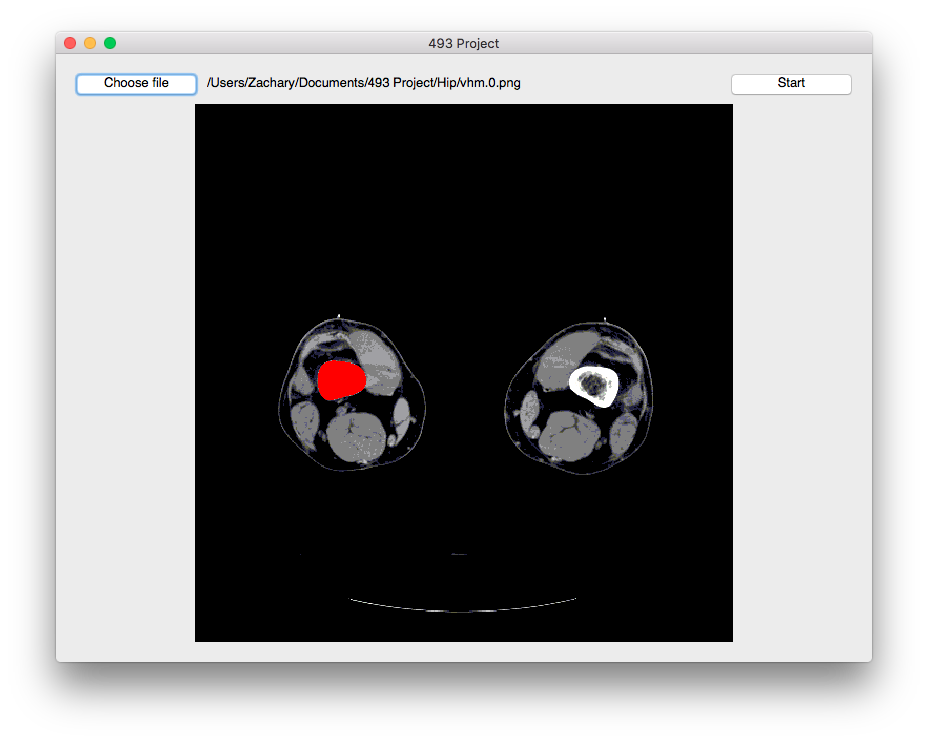
\includegraphics[width=1\textwidth]{python}
      \label{python_implementation}
        \end{figure}
        
    \subsection{C++ Implementation}
    As alluded to earlier, speed is a critical component to implementing this region tracking algorithm in a real world context. Speed is positively related with all components of the triple bottom line. In the medical imaging domain, if the application runs efficiently it is associated with reduced costs, improved segmentation which might yield better treatment to patients, and a reduced ecological footprint due to lower power consumption. Thus, a C++ implementation was completed to replicate a practical implementation of this algorithm. It was also beneficial to make a GUI for the application as it would assist in testing and verification of the algorithm. It would allow any user to quickly change parameter values and test different combinations of the functionals based on the attributes of their image sequence. To aid in the development of the GUI, the Qt framework and the Qt Creator IDE was used (\url{http://www.qt.io/}).
    
    By looking at the code base (\url{https://github.com/WillMueller/Thesis/tree/master/CImplimentations}) the C++ structure mirrors that of the Python implementation. The two main files and their associated headers are mainwindow..cpp and levelset.cpp. The first file is the business logic of the GUI and uses levelset.cpp to apply the algorithm to the user's inputs. The second file implements a standalone class that performs the algorithm in a series of steps. In the first step, initialization, the user creates the object by giving it an initial image with a highlighted region. Next, they set the parameter values of the functionals and the number of iterations for the gradient descent. Finally, they run the algorithm. In the context of the GUI, these steps are formalized in Figure \ref{cpp_implementation} and the subsequent bullet list.
    
    \begin{figure}[!ht]
      \caption{C++ GUI Implementation}
      \centering
      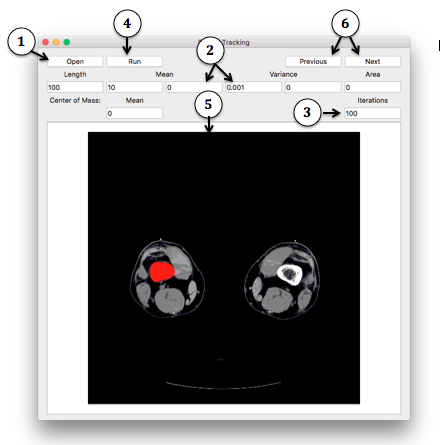
\includegraphics[width=0.8\textwidth]{c++}
      \label{cpp_implementation}
    \end{figure}
    
    Steps the user takes to utilize the application:
    \begin{enumerate}
    	\item Open the initial image with the region of interest highlighted in red. The images must be in the same directory and have the format X.1.png, X.2.png,..., X.N.png. Where X can be any string and N is the number of images. The user is not restricted to using PNG's and can use any of the popular image extensions (.jpg, .png, .bmp, etc.).
        \item Decide which functionals to use and set the parameter values in the text fields. Note that there are two fields for mean and variance as it can be applied to both the inside and outside of the region.
        \item Decide on the number of iterations the gradient descent should perform on each image.
        \item Run the region tracking algorithm.
        \item As the algorithm runs, it will output each image with the region highlighted in blue after the defined number of iterations is run.
        \item After the algorithm has been applied to every image in the sequence, the user can flip through each image and see how the region evolves over the sequence.
	\end{enumerate}    
    
    There are a couple of things to note with the C++ implementation. First, we wanted to simulate a real world application as closely as possible. Mathematically, we know the gradient descent will eventually reach some critical point given enough iterations. However, in a pragmatic setting, it is unfeasible to wait for that many iterations. Hence, we chose to default the number of iterations to 100 as this produced a reasonable computation time on consumer grade hardware. At 100 iterations, the time to process a single image was measured in tens of seconds. For the medical image domain, where image sequences range in the hundreds, this equates to a few hours of computation time. Depending on the urgency of the case, this competes directly with the time it would take humans. This justified the use of 100 iterations as a realistic number to compare this algorithm's ability against ground truth. The last thing to note is the speedup realized by the conversion to a C++ implementation. Keeping everything else constant, the conversion to C++ yielded an increase in performance by 400-500\%. This turned simulations that took a day into one that took several hours.

	\section{Results}
		
		\subsection{Final Performance on Medical Images}
		The results of the algorithm using the final optimized parameters are shown in Figures \ref{fig:hip4_25}, \ref{fig:hip4_350}, and \ref{fig:hip4_375}. 
		\begin{figure}[H]
			\centering
			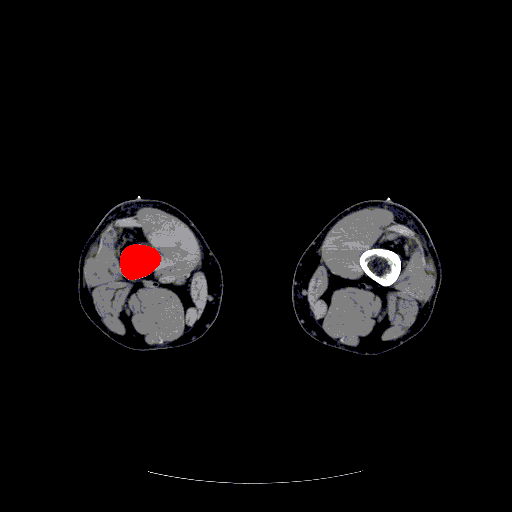
\includegraphics[width=0.4\textwidth]{Hip4/groundTruth25col.png}
			\hspace{20pt}
			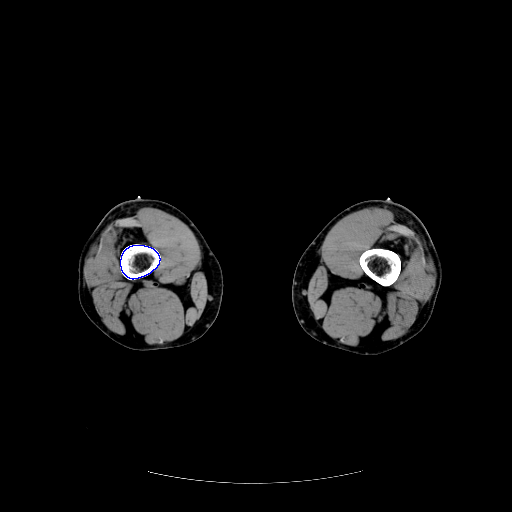
\includegraphics[width=0.4\textwidth]{Hip4/output25.png}
			\caption{Hip image 25 -- ground truth (left) compared to algorithm output with final parameter set (right).}
			\label{fig:hip4_25}
		\end{figure}
		\begin{figure}[H]
			\centering
			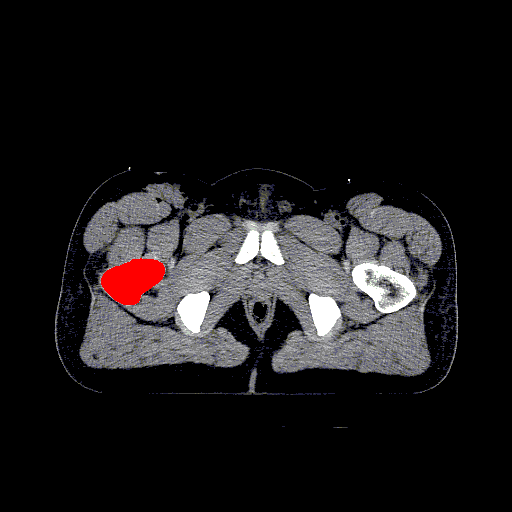
\includegraphics[width=0.4\textwidth]{Hip4/groundTruth350col.png}
			\hspace{20pt}
			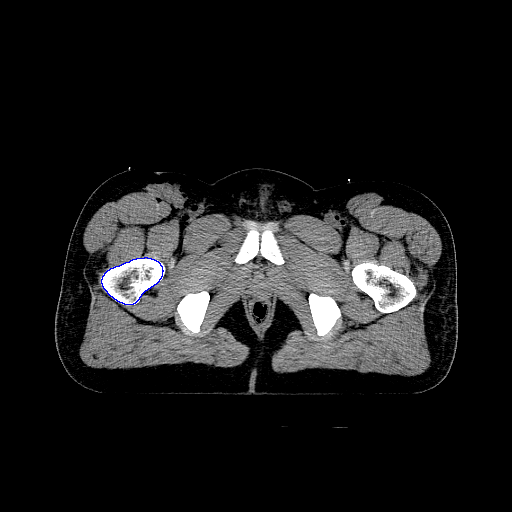
\includegraphics[width=0.4\textwidth]{Hip4/output350.png}
			\caption{Hip image 350 -- ground truth (left) compared to algorithm output with final parameter set (right).}
			\label{fig:hip4_350}
		\end{figure}
		\begin{figure}[H]
			\centering
			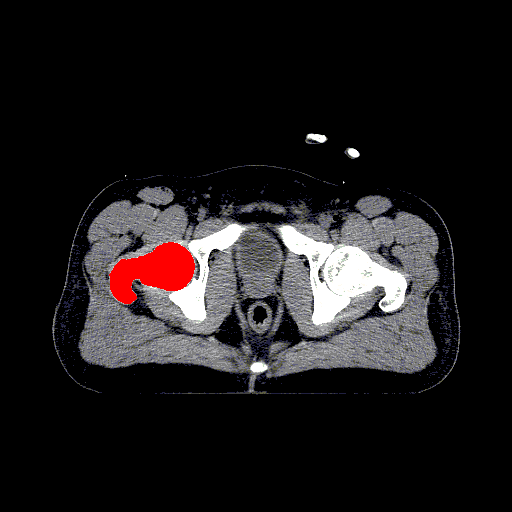
\includegraphics[width=0.4\textwidth]{Hip4/groundTruth375col.png}
			\hspace{20pt}
			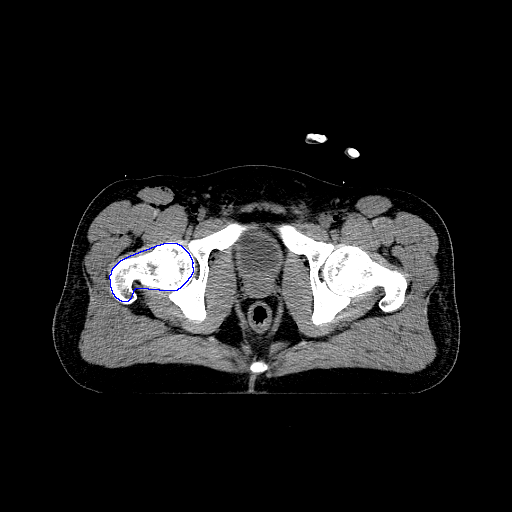
\includegraphics[width=0.4\textwidth]{Hip4/output375.png}
			\caption{Hip image 375 -- ground truth (left) compared to algorithm output with final parameter set (right).}
			\label{fig:hip4_375}
		\end{figure}
		On image 25 (Figure \ref{fig:hip4_25}), the algorithm incorrectly identified 4.13\% of the image pixels by volume of the ground truth. This corresponds to an incorrect identification of 0.017\% of the image pixels over the entire image. As the algorithm proceeded to subsequent images, the error rate did not increase significantly until the shape of the hip bone changed drastically around the \nth{375} image. This is evidenced by the similar error rate obtained in image 350 (Figure \ref{fig:hip4_350}) compared to image 25. In image 350, the percentage of erroneous pixels was 3.82\% of the volume of the ground truth, and 0.041\% of volume of the entire image. However, by image 375 (Figure \ref{fig:hip4_375}), these error rates increased to 13.12\% and 0.17\%, respectively.

		Overall, the algorithm error rate with these final parameters was averaged over the \nth{25}, \nth{75}, \nth{350}, and \nth{375} images. Due to the amount of manual work required to determine ground truth, the evaluation of the algorithm could only be measured over a subset of the images. The images near the beginning and the end of the sequence were assumed to be most revealing of algorithm performance due to gradual shape changes in this dataset. Over this subset, the average error rate as a fraction of ground truth was 6.00\%. The average error rate as a fraction of the entire image was 0.056\%. While we were aiming to have the average error rate over ground truth lower than 5\%, so the algorithm's final performance did not quite reach our expectations in this regard. However, we were also targeting for our algorithm to have less than a 0.1\% error rate over the entire image region, and it outperformed in this metric. See Section \ref{sec:futurework} for areas where the algorithm could have been improved to lower the error rate.
		
		\subsection{Final Performance on Hand Gesture Images}
	\section{Discussion (3bottom)}
		Mandy

	\section{Conclusion}
	\section{Future Work} \label{sec:futurework}
		Faisal
	\nocite{*}
	\bibliographystyle{plain}
	\bibliography{bibliographyExample}
	
\end{document}
